\documentclass[a4paper,12pt]{article}
\usepackage[utf8]{inputenc}  % Denna rad är datorspecifik
\usepackage[swedish]{babel}
\usepackage{fancyvrb} % Ger ramar runt verbatimblock

\title{\LaTeX\ och prov D1:\emph{Snöflingan} \\
       D om texter och \LaTeX i kursen D0015E} 

\author{Håkan Jonsson\\ ~\\ Institutionen för system- och
  rymdteknik \\ Luleå tekniska universitet}

\begin{document}

\maketitle

\begin{abstract}
  Prov D1:Snöflingan går ut på att skapa ett dokument identiskt med
  ett annat med hjälp av \LaTeX. Här ges en förklaring till innehållet
  i den startfil  du får.  
\end{abstract}

\section{Allmänt}

\LaTeX\ erbjuder fantastiska möjligheter att producera professionellt
typsatt text, men också lika stora möjligheter att göra fel. Du måste
därför vara \emph{mycket noggrann} då du skriver ditt
\LaTeX-manus. Minsta tecken har betydelse och även små fel, som att
råka använda en stor bokstav där det ska vara en liten, gör att varje
försök att generera ett dokument från manuset rasar samman som ett
korthus.
%
\begin{center}
  \noindent
  \fbox {
    \parbox{0.8\textwidth}{
      Skriv manuset i mycket små steg och generera dokument mellan
      stegen, så får du eventuella fel i småportioner och kan enklare
      åtgärda dem. Jag gör alltid så här och jag råder även dig att
      göra det. 
    }
  }
\end{center}

\subsection{Layout}

Skilj mellan \emph{innehåll} och \emph{utseende}. Koncentrera dig på
innehållet, dvs att text och formler får korrekt innehåll, och överlåt
sen åt \LaTeX\ att bestämma utseendet. Kanske detta känns ovant, för
WYSIWYG\footnote{What-You-See-Is-What-You-Get.}-program som t ex
Microsoft~Word bygger ju på att skribenter också bestämmer
layouten. Men \LaTeX\ är inte något WYSIWYG-program. \LaTeX\ är
programmerat med hjälp av de bästa layoutreglerna och layoutar bättre
än oss alla i 99 fall av 100.

Om du trots allt till slut tycker att layouten inte är bra så vänta
med uttryckliga ändringar av den tills du fått allt innehåll
korrekt(!) Alltså:

\begin{itemize}
  \item Först se till att allt innehåll finns inknappat och går att
    generera pdf från utan att det blir särskilt snyggt.
  \item Sen jobba med hur layouten blivit. 
  \end{itemize}
  
Annars skapar du bara en massa problem för dig själv. Även små
ändringar av innehållet kan orsaka mycket stora ändringar av hur
\LaTeX\ utformar dokumentets layout. 

\subsection{Kommentarer}

\LaTeX-systemet ignorerar allt på en rad efter ett procenttecken
(\verb!%!). Med \verb!%! kan man således inkludera kommentar i sitt
manus som inte påverkar det färdiga dokumentet men som kan vara
viktiga för någon som läser manuset.
% Här är en kommentar som du som läsare av manuset kan se men som inte
% syns i den färdiga pdf:en.  

\subsection{Kommandon och omgivningar}

Ett \LaTeX-kommando startar med ett bakåt-snedstreck (\verb!\!). Sen
följer kommandots namn och eventuella argument\footnote{Jämför med hur
funktioner och metoder används i programmeringsspråk som
\texttt{python}.}. Vill man t ex ha \textbf{text med fet stil}
använder man kommandot \label{sec:textbf}
\verb!\textbf{text med fet stil}!. Vill man istället att \emph{text 
ska framhävas} så skriver man \verb!\emph{text ska framhävas}!.
\label{sec:emph} Det finns väldigt många olika kommandon 
och ett råd är att snarare googla efter/slå upp detaljer då du behöver
dem än att lära dig dem alla utan till.  

Förutom kommandon finns det även \LaTeX-omgivningar
(\textit{environments} på engelska). Dessa inleds med \verb!\begin!,
  avslutas med \verb!\end! och påverkar det som skriv mellan
\texttt{begin-end}. Exempel: Om man vill 
%
\begin{center}
  centrera text så här
\end{center}
%
använder man omgivningen \texttt{center} och skriver
%
\begin{verbatim}
\begin{center}
  centrera text så här
\end{center}
\end{verbatim}
%
Om du läser manuset till detta dokument kommer du att se att jag
använt omgivningen \texttt{verbatim} för att får in
centreringsomgivningen ovan i min text.  

\subsection{Tomrum}

En \emph{tomrad} (eller flera efter varandra) bland text markerar
\emph{nytt stycke}.

Detta kan märkas genom att första raden dras in eller att \LaTeX\
lägger in lite tomrum vertikalt mellan styckena. Var noga med
eventuella tomrader du väljer att ta med i ditt manus.

Däremot spelar godtyckligt många mellanslag mellan ord i text ingen
annan roll än att de byts ut mot ett lagom stort mellanrum oavsett hur
många de är. Därför kan man i regel fritt \emph{indentera rader}, dvs
stoppa in mellanslag i början av rader för att visa på hur på varandra
följande rader hör ihop, och därigenom dramatiskt öka manusets
läsbarhet. 
%
\begin{center}
  \noindent
  \fbox {
    \parbox{0.8\textwidth}{
      Jag brukar indentera sånt som är inne i en omgivning minst 2
      mellanslag relativt närmast omgivande omgivning. Det gör att jag
      enklare ser vad som tillhör vad. Om jag inte hinner indentera
      när jag skriver så återvänder jag till texten och gör det
      senare. Jag råder dig att indentera på samma sätt som mig, och
      även då du programmerar datorer. I vissa språk, t ex
      \texttt{python}, har indenteringen även betydelse för
      slutresultatet.  
    }
  }
\end{center}

\section{En genomgång av \texttt{koch-start.tex}}

Här följer nu en genomgång av startfilen \texttt{koch-start.tex} som
du ska utgå från. Uppgiften är att lägga till text och kod. Du behöver
inte ta bort något, utan allt i filen ska vara kvar.

\subsection{Inledningen}

\begin{Verbatim}[frame=single]
\documentclass[12pt,a4paper]{article}
\usepackage[utf8]{inputenc}
\usepackage{graphicx}
\usepackage{amsmath, amsthm, amssymb}
\usepackage[a4paper,includeheadfoot,margin=2.54cm]{geometry}
\newtheorem{theorem}{Theorem}
\end{Verbatim}

Varje \LaTeX-manus inleds med lite allmänna deklarationer och
importer, och så är också fallet med detta manus.  

\begin{itemize}
  \item \verb|\documentclass[12pt,a4paper]{article}| säger att detta
    är ett manus för en artikel som ska typsättas med 12 punkters 
    typsnitt och passa på ett A4-ark. 

  \item \verb|\usepackage[utf8]{inputenc}| anger den teckenkodning som
    används. Detta är datorspecifikt så du kan behöva ändra
    \texttt{uft8} till något annat t ex \texttt{latin1}.  

    \verb|\usepackage| är ett kommando som importerar andra kommandon
    och omgivningar än de som det grundläggande \LaTeX-systemet består
    av. Kommandot gör det importerade tillgängligt när man skriver
    manuset. 

  \item \verb|\usepackage{graphicx}| gör det möjligt att inkludera
    grafik, t ex JPEG-bilder eller PDF-filer. Detta gör man i
    praktiken sen med kommandot \verb|\includegraphics|. 

  \item \verb|\usepackage{amsmath, amsthm, amssymb}| utökar stödet för
    matematik. 

  \item Den långa raden
    \verb!\usepackage[a4paper,includeheadfoot,! \\ 
        \verb!margin=2.54cm]{geometry}! förtydligar att sidorna ska ha
        marginal på 2.54mm (1 tum).

        % Kommandot verb är lite speciellt och typsätts inte på
        % normalt sätt. Detta är varför jag radbryter med \\
        % ovan. Utan radbrytningen hamnar en del ute i marginalen och
        % t o m utanför papperet. Sån radbrytning ska man generellt
        % sett undvika om man kan för den kan förstöra LaTeX:s egen
        % typsättning. 
        
  \item \verb|\newtheorem{theorem}{Theorem}| introducerar
    \texttt{theorem}, en ny omgivning för matematiska satser/teorem. 
\end{itemize}

Inledningen kan även definiera titel, författarnamn, datum,
rubrikstilar och annat. Men så görs inte här. Inledningen ovan ska
vara som den är, dvs du ska inte ändra i den. 

\subsection{Resten av manuset} \label{resten}

Här följer nu en genomgång, rad för rad, av resten av
\texttt{koch-start.tex}. Denna genomgång gör det lättare för dig att
komplettera manuset och få det rätt. 

\begin{Verbatim}[frame=single]
\begin{document}
\end{Verbatim}
% 
Börjar beskrivningen av dokumentinnehållet. Allt som skrivs mellan
denna rad och raden \verb!\end{document}! i slutet av manuset, och i
den ordning det skrivs (uppifrån och ned, vänster till höger), anger
dokumentinnehåll, dvs text blandad med kommandon som säger vad
textdelarna är för något. 

\begin{Verbatim}[frame=single]
\section{The Koch Snowflake}
\end{Verbatim}
%
Att använda \verb|\section| ger en automatnumrerad
huvudrubrik. Argumentet till kommandot, i detta fall \texttt{The Koch
  Snowflake}, är rubriktexten. \LaTeX\ kommer att välja en lagom
storlek på rubriken som passar till det slutgiltiga dokumentets
storlek och text.   

\begin{Verbatim}[frame=single]
The \emph{Koch snowflake},
\end{Verbatim}
%
Med \verb|\emph| markeras \emph{betonad} text.  

\begin{Verbatim}[frame=single]
Helge von Koch~\cite{koch}.  
\end{Verbatim}
%
\verb|\cite| används för att referera till en referens, som beskrivs i
omgivningen \texttt{thebibliography} i slutet av manuset. En referens
är typiskt en artikel eller rapport. Här refererar vi referensen
\texttt{koch}, vilket är varför vi skriver \verb|\cite{koch}|. \LaTeX\
kommer att byta ut \verb|\cite{koch}| mot ett löpnummer inom
hakparenteser. 
    
Har man flera referenser ger \LaTeX\ varje ett eget nummer och ser
till att utbytena blir rätt. Detta är mycket smidigt eftersom man inte
själv behöver hålla reda på löpnumren, utan kan helt överlåta detta åt
\LaTeX-systemet. Däremot måste man (förstås) själv definiera
referenserna och ge dem unika nyckelord (i detta fall \texttt{koch}). 

Notera det lilla vågtecknet (\verb!~!) i \verb!Koch~\cite!. Detta är
nödvändigt för att förhindra radbrytning just där. Utan detta tecken
finns risk att referensen inom hakparanteser, som \LaTeX\ skapar och
lägget in, annars skulle kunna hamna först på ny rad. Sån typsättning
vore fel (och ful).  

\begin{Verbatim}[frame=single]
\begin{figure}[h] \label{koch}
\end{Verbatim}
%
\verb|figure| är en omgivning för figurer som man vill ha bildtext
till, t ex bilder. \verb|[h]| anger att vi vill ha figuren just
\textbf{h}är, och inte någon annanstans(!) Beroende på \LaTeX:s
layoutregler \emph{kan} figuren ändå hamna på annan plats, vilket man
då kan åtgärda. Men sådan åtgärd ska man alltså vidta först när allt
annat innehåll är korrekt (inte omedelbart när man till sin fasa ser
att figuren hamnar på fel ställe).   

\verb|\label| är en etikett för något i dokumentet som man sen vill
kunna referera till som avsnitt, ekvationer, sidor, bilder, tabeller
mm. Till \verb|\label| fogar man ett unikt namn på etiketten som man
sen känner igen. En etikett för ett inledande avsnitt skulle kunna
vara \verb|sec:intro| medan man för en ekvation kanske använder
\verb|eq:pythagoras|. De här prefixen \texttt{sec:} och \texttt{eq:}
är inget \LaTeX-systemet kräver, utan bara till för att man snabbt ska
se vad för något en referens leder till. För en figur brukar jag
skriva t ex \verb|\label{fig:circle}|, där \texttt{fig:} gör det lätt
att skilja etiketten från etiketter för avsnitt och ekvationer. Du får
döpa dina etiketter som du vill men håll dig till vanliga bokstäver i
etikettnamnen.  
   
Avsnitt, ekvationer, figurer och annat numreras separat inom
respektive sort och stigande. Det går dock att ändra detta (men det
behöver man sällan).  

\begin{Verbatim}[frame=single]
  \centering
\end{Verbatim}
%
\verb|\centering| inne i en \texttt{figure} ger centrering av
figuren. Omgivningen \texttt{center} fungerar likartat men ska inte
användas just här.  

\begin{Verbatim}[frame=single]
  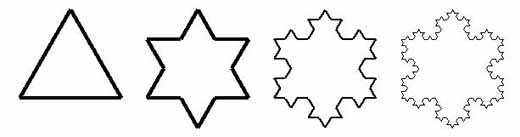
\includegraphics[width=10cm]{snowflake.jpg}
\end{Verbatim}
%
Kommandot \verb|\includegraphics| säger att här ska grafik in från en
fil vars namn ett argument anger. Vår fil heter \texttt{snowflake.jpg}
och dessutom före\-skriver vi att vi vill att bilden får en bredd på 10
cm. \LaTeX\ kommer då att skala om bilden så den får bredden 10 cm och
behåller sina proportioner.

Skriver man istället \verb!width=\textwidth! skalas bilden istället om
så den blir lika bred som texten. Man kan skippa att ange en bredd men
då får bilden sin naturliga bredd (oskalad), vilket ofta ser dåligt ut. 

Bilder är något \LaTeX\ inte klarar av särskilt väl. Bildhantering i
\LaTeX\ är krångligt, blir ofta fel, och därför har jag inkluderat
hela det kommando du ska använda för att få in bilden  på snöflingans
första konstruktionssteg.  

\begin{Verbatim}[frame=single]
  \caption{The Koch snowflake }
\end{Verbatim}
%
\verb|\caption| anger helt enkelt en bildtext.

\begin{Verbatim}[frame=single]
\end{figure}
\end{Verbatim}
%
Varje omgivning börjar med \texttt{begin} och måste avslutas med
\texttt{end}, och här avslutas således \texttt{figure}-omgivningen.

\begin{Verbatim}[frame=single]
infinite number of times:
\begin{quote}
  \textit{Divide.}
\end{quote}
\end{Verbatim}
%
Omgivningen \texttt{quote} lägger in ett längre citat, och indenterar
\emph{lagom mycket} från både höger och vänster. \verb|\textit| ger
kursiv stil.  

\begin{Verbatim}[frame=single]
Figure~\ref{koch}.
\end{Verbatim}
%
Kommandot \verb|\ref| används för att referera till något i dokumentet
som märkts ut med en etikett. Om man t ex lagt in en (enda) figur/bild
i sitt dokument, och i denna inkluderat etiketten \verb|\label{koch}|,
så kommer \verb|\ref{koch}| i texten sen att bytas ut mot
\verb![1]!. Skulle figuren vara den andra figuren i ordning, sker
utbytet istället till \verb![2]! osv. 

\begin{Verbatim}[frame=single]
\begin{theorem}
  infinite length. 
\end{theorem}
\end{Verbatim}
%
Omgivningen \texttt{theorem} typsätter en matematisk sats (ett
teorem).  

\begin{Verbatim}[frame=single]
\begin{proof}
\end{Verbatim}
%
Efter \texttt{theorem}, ett matematiskt påstående, passar det med ett
bevis av påståendet. Det är vad omgivningen \verb|proof| används
för. I ditt manus ska du skriva kod för två bevis (ja, även två
teorem) som alltså läggs in i omgivningen \verb|proof|. Notera att
\texttt{proof} automatiskt lägger till en passande slutsymbol.   

\begin{Verbatim}[frame=single]
  $\Delta$
  $N_i$ 
  $L_i$
\end{Verbatim}
%
Matematisk löptext märks i \LaTeX\ ut genom att omges av dollartecken
(\verb|$|). Skriver man t ex \verb|$f(x)+f(2x)/2+f(3x)/3$| typsätts
det som matematisk text, dvs 
%
\begin{displaymath}
  f(x) + f(2x) / 2 + f(3x) / 3,
\end{displaymath}
%
och inte som vanlig text, dvs f(x) + f(2x) / 2 + f(3x) / 3. Lägg noga
märke till stilskillnaden. Skilj noga mellan vad i manuset som är
vanlig text och vad som är matematik. Det är fel att typsätta
matematik, t ex variabler, som vanliga text. 

\verb|\Delta| ger den grekiska bokstaven stora D~(dvs
$\Delta$). \verb|N_i| och \verb|L_i|  ger i matematisk text $N_i$
respektive $L_i$. Rent generellt ger understrykningstecken (\verb!_!)
ett \emph{index} i matematisk text. 

\begin{Verbatim}[frame=single]
  Then
  \begin{displaymath}
\end{Verbatim}
%
\verb|displaymath| ger en formel som typsätts fritt i ett  större
vertikalt mellanrum. Man behöver inga dollartecken i omgivningen, utan
\LaTeX\ förutsätter att det som skrivs där måste vara matematik.  
    
Samma matematiska text kan i regel antingen typsättas i löptext, med
dollartecken, eller fritt med bl a \texttt{displaymath}; se även
\texttt{equation} nedan.   

\begin{Verbatim}[frame=single]
    =
    \begin{cases}
      3, & \text{if $n=0$ } \\
    \end{cases}
\end{Verbatim}
%
\verb|cases| används för ekvationer med många fall. Koden
\verb|\text{en mening}| i matematiska formler gör att \texttt{en
mening} typsätts som vanlig löptext, inte som matematik. Detta är
användbart när man vill lägga till förklaringar eller villkor (som här
där värdet i första fallet är 3 men endast om $n=0$).

Sekvensen \verb!\\! betyder att här ska en radbrytning alltid in. Så
måste man skriva i en del matematikomgivningar (t~ex~\texttt{cases})
men annars ska man endast använda det sparsamt och försiktigt. Det
förstör nämligen \LaTeX:s egen typsättning och ger (oftast) ett fult
resultat.  

\begin{Verbatim}[frame=single]
  \end{displaymath}
\end{Verbatim}
%
Detta avslutar mera luftig typsättning av matematik. 

\begin{Verbatim}[frame=single]
  This 
  \begin{equation}
    \label{eq:1}
    \cdot
  \end{equation}
\end{Verbatim}
%
Omgivningen \verb|equation| används som \texttt{displaymath} men ger
automatiskt ett ekvationsnummer som skrivs ut i marginalen. Koden   
%
\begin{verbatim}
\begin{equation}
  \label{eq:first}
  f(x) = x^2 + 2x + 9
\end{equation}
\end{verbatim}
%
ger t ex 
%
\begin{equation}
  \label{eq:first}
  f(x) = x^2 + 2x + 9
\end{equation}
%
och refererar man sen till etiketten \texttt{eq:first} med
\verb!Eq.~\ref{eq:first}! gör \LaTeX\ om detta till  
%
\begin{quote}
  Eq.~\ref{eq:first}
\end{quote}
%
Som tidigare påpekats är den ''våg'' (\verb|~|) som syns i koden (och
som även kallas \emph{tilde}) ett fast mellanslag, ett slags klister
som beordrar \LaTeX\ att behandla det ihopklistrade som ett ord. Detta
används för att hindra radbrytning mellan Eq. och siffran
\ref{eq:first}. I just detta sammanhang, precis som för \verb!\cite!,
får radbrytning inte ske, och \LaTeX\  måste då upplysas om det. 

\verb|\cdot| ger en centrerad punkt i matematik. En sådan brukar
användas för att visa multiplikation mellan två tal eller där man
annars vill trycka på att det verkligen är multiplikation. Annars ska
man aldrig använda en punkt för multiplikation. Alltså, man skriver
$f(x)g(x)$ och inte $f(x)\cdot g(x)$. Däremot måste man skriva $3\cdot
4$ för annars blir det $34$, dvs ett tal och inte en multiplikation.  

\begin{Verbatim}[frame=single]
   while  
  \begin{equation}
    \label{eq:5}
    L_n = \frac{L_{n-1}}{3} =.
  \end{equation}
\end{Verbatim}
%
Kommandot \verb!\frac! ger ett bråk. Ovan är $L_{n-1}$ täljare och $3$
nämnare.

\verb|L_{n-1}| gör hela uttrycket $n-1$ till index. Klammerparenteser
kan alltid användas för att gruppera ihop uttryck som (bland annat)
index. Skriver man t~ex \label{sec:maas} 
%
\begin{center}
  \verb|$B_{N_{i+1}+M_{j+2i}}$|
\end{center}
%
får man 
%
\begin{displaymath}
  B_{N_{i+1}+M_{j+2i}}.
\end{displaymath}

Observera att \verb|\frac| ofta passar mindre bra i löptext, då allt
kan se högst ihoptryckt ut: Koden \verb! $\frac{L_{n - 1}}{3}$! ger
$\frac{L_{n - 1}}{3}$. Då kan man ofta få finare text genom att
använda ett helt vanligt snedstreck: $L_{n - 1}/3$. 

\begin{Verbatim}[frame=single]
  From Eqs.~\ref{eq:1}  
\end{Verbatim}
%
Återigen nödvändig användning av tecknet \verb!~!. 

\begin{Verbatim}[frame=single]
  \begin{displaymath}
    N_nL_n =
    \left(      \right)
    .
  \end{displaymath}
  it follows $\to \infty$, which. 
\end{Verbatim}
%
\verb|\left| och \verb|\right| ger storleksanpassade
parenteser. Skriver man
%
\begin{center}
  \verb|( \frac{4}{3} )|
\end{center}
%
får man 
%
\begin{displaymath}
  ( \frac{4}{3} )
\end{displaymath}
%
medan \verb|\left( \frac{4}{3} \right)| ger det betydligt snyggare 
%
\begin{displaymath}
  \left( \frac{4}{3} \right)
\end{displaymath}
%
Istället för parenteser kan man använda annat t ex klammerparenteser
eller hakparenteser. \verb|\left[ \frac{4}{3} \right]| skulle t~ex~ge  
%
\begin{displaymath}
  \left[ \frac{4}{3} \right]
\end{displaymath}
%
Observera att \verb|\left| och \verb|\right|
alltid förekommer i par. Punkt som parentestecken gör att inget
parentestecken skrivs ut. Detta kan användas både efter \verb!left!
och \verb!\right!. \verb|\left\{ \frac{4}{3} \right.| skulle t~ex~ge  
%
\begin{displaymath}
  \left\{ \frac{4}{3} \right.
\end{displaymath}
%
(Av tekniska skäl måste man skriva \verb!\{! om man menar en
klammerparentes, tecknet alltså, för \verb!{! och \verb!}! används ju
för att skriva kommandon och omgivningar.)

\verb|\to| ger en högerpil och \verb|\infty| ger tecknet $\infty$,
oändligheten. 

\begin{Verbatim}[frame=single]
\end{proof}
\end{Verbatim}
%
Beviset är klart och med \verb! \end{proof}! avslutas det med en
symbol till höger. 

\begin{Verbatim}[frame=single]
  The Koch snowflake has finite area. 
\end{Verbatim}
%
Ett nytt teorem inleder den andra delen av dokumentet. Till detta ska
fogas ett bevis.  

\begin{Verbatim}[frame=single]
  In an iteration,, the number of new triangles $T_n$, 
  Eq.~\ref{eq:1}, 
  can be simplified to 

    \label{eq:2}
\end{Verbatim}
%
Början på beviset. 
 
\begin{Verbatim}[frame=single]
  $a_n$
  \begin{displaymath}
    a_0=
  \end{displaymath}
\end{Verbatim}
%
Notera att i matematikomgivningar behövs inga dollartecken.
\verb|\sqrt| ger kvadratroten ur något. \verb|$\sqrt{x}$| blir
$\sqrt{x}$. 

\begin{Verbatim}[frame=single]
  $\Delta$, the initial equilateral triangle,, or 
  \begin{equation}
    \label{eq:3}
    a_n = \frac{a_{n-1}}{9} = \ldots .
  \end{equation}
\end{Verbatim}
%
\verb|\ldots| ger tre punkter på textens baslinje och används för att
markera att något utelämnats.  

\begin{Verbatim}[frame=single]
  Eqs.~\ref{eq:2} and \ref{eq:3}
  \begin{equation*}
\end{Verbatim}
%
Omgivningen \verb|equation*| fungerar som \texttt{displaymath}.

\begin{Verbatim}[frame=single]
    b_n = = \left( \cdot 4^n \right) \left( a_0 \right)  =. 
  \end{equation*}
\end{Verbatim}
%
 Tecknet \verb|^| ger ''upphöjt i'', dvs en exponent i matematisk
 text. Exempel: Att skriva \verb|$x^{f(x)}$| ger $x^{f(x)}$.  Notera
 att du alltså kan använda klammerparenteser för att grupera ihop hela
 uttryck som exponenter på samma sätt som du ovan tidgare kunde
 använda dem för att ha uttryck som index~(se
 sidan~\ref{sec:maas}).

 Har man en enkel exponent behövs inga klammerparenteser. För att få
 $x^2$ räcker det att skriva \verb|$x^2$|.  

\begin{Verbatim}[frame=single]
  total area
  \begin{align*}
    A &= a + \sum_{k=1}^n b \\
      &= a_0\left(1 + \left( \right)^k \right) \\
      &= .
   \end{align*}
\end{Verbatim}
%
Omgivningen \verb|align*| är till för ekvationer som går över
många led och rader. Notera hur \verb!\\! används i \texttt{align*}
för att avsluta rader/fall. Raderna justeras i förhållande till
varandra så att de tecken som följer efter \verb!&!-tecknen (i detta
fall likamedtecken) hamnar under varandra.  

\verb|\sum| ger ett summatecken i matematisk text. Om man ger
\LaTeX-koden 
\verb|\sum_{k=1}^n b_k| får man t ex $ \sum_{k=1}^n b_k$ i löptext
och   
%
\begin{displaymath}
  \sum_{k = 1}^n b_k
\end{displaymath}
%
i mera luftig text.
    
\begin{Verbatim}[frame=single]
  Now, since
  \begin{displaymath}
    \lim_{n} 3\left( \right) = 0,
  \end{displaymath}
\end{Verbatim}
%
Kommandot \verb|\lim| används för gränsvärden. Skriver man t ex
%
\begin{center}
  \verb!\lim_{x \to \infty} \frac{1}{x} = 0!
\end{center}
%
blir det $\lim_{x \to \infty} \frac{1}{x} = 0$ i löptext och 
%
\begin{displaymath}
  \lim_{x \to \infty} \frac{1}{x} = 0
\end{displaymath}
%
i en \texttt{displaymath}. 

\begin{Verbatim}[frame=single]
  $\lim_{\to \infty} A_n$..  
\end{Verbatim}
%
Samma här. 

\begin{Verbatim}[frame=single]
\begin{thebibliography}{99}
\end{Verbatim}
%
\verb|thebibliography| är en omgivning som bygger upp en referenslista
där varje referens anges med hjälp av kommandot \texttt{bibitem}. Det
är dessa som sen refereras till med kommandot \verb!\cite!. 

\begin{Verbatim}[frame=single]
  \bibitem{koch} Helge. \emph{Sur une courbe continue sans
      tangente, obtenue par une construction géométrique
      élémentaire.}, Arkiv,
    Kungliga Vetenskapsakademien. \textbf{1}, 681-702,.
\end{Verbatim}
%
En referens (den enda i dokumentet). Kommandot \verb|\textbf| ger fet
stil.  

\begin{Verbatim}[frame=single]
\end{thebibliography}
\end{Verbatim}
%
Avslutar referenslistan.

\begin{Verbatim}[frame=single]
\end{document}
\end{Verbatim}
%
Avslutar hela manuset. 
\end{document}
